\section*{Verification}
In the previous sector we talked about what tools could be possibly be used in order to analyze and perform other tasks in a Petri Net. In this section we present more information about the task of verification and the challenges that creates.

Currently the are three major problems with the task of \emph{verification}. We emphasize in the problems of reachability, liveness and the existence of deadlocks. As you can easily understand there is a number of embedded devices and other possible targets the meaning of safe operation is becoming very important and can not be avoided. Try to imagine the meaning of safety in the context of Web services, we must be able to verify that a composite service upholds a certain amount of a safety for each constraint. For example, we must make sure that when a financial transaction takes place using a Web service, very common in nowadays, the charge happens only once and the bought products are being send off only the corresponding times there were bought. In the same logic we are evaluating the verification of safety constraints, the detection of deadlocks and that the actual automated composition of these Web services is being done in terms of reachability.

In order to do that we try to define those principles in the same way we did in the prior work presented in this work.

\begin{description}
\item[Reachability] A marking M is reachable if it is the marking reached by some occurrence sequence (Definition 4). Given a marking M of N, the set of reachable markings of the net (P; T; F; M) (i.e., the net obtained by replacing the initial marking M0 by M. Notice that the empty sequence is an occurrence sequence and that it reaches the initial marking M0. The reachability problem for a net N is the problem of deciding for a given marking M of N if it is reachable. With the above knowledge we can try and define the meaning of \emph{safety}.

\textbf{Safety} of a distributed system is defined as lack of reachability to an unsafe state

\item[Safety of Web Service Compositions] Let S be a Web service composition with associated net (P;T;F;M). Let $\phi$ be a safety constraint, and let marking M’ encode the negation (i.e., the violation) of the safety constraint $\phi$. Then a Web service composition S is safe with respect to $\phi$ iff there is no occurrence sequence of the net of S that reaches M’.

In a similar way we define the task of generating a composition of Web services to achieve a goal as the problem of finding an occurrence sequence that reaches the marking depicting the user's desired final state. In order to do that we can use a composition of atomic services to achieve the final target state.

\item[Automated Composition of Web Services] Let A be a set of atomic Web services and let N=(P;T;F;M) be the net that depicts the behavior of all the services in A. Further, let $\phi$ represent the user’s goal, and let M’ be the marking that depicts this goal in N. Then a1;a2,...;an is a sequential composition of atomic services that achieves user goal $\phi$ iff a1;a2,...;an is an occurrence sequence in the reachability analysis of M’ in N. In the case of the composition of a Web service we consider it as an individual service treated as an atomic process. Also, it is important to remember that a smart agent given an agent goal, a service description and our process semantics can produce the optimal composition of using partial service executions.

The idea of using the feature of automated composition for the Web services is analogous of an AI to design systems where we have all the necessary informations from the beginning. Finally, it is essential to remember that in most real life and practical Web services the possible compositions are very branchy and offer many options, but on the final resulting composition tend to be short and the most efficient.
\end{description}

\subsection*{Complexity of DAML-S services tasks}
Below we present the complexity of each DAML-S approach. This is important in the case the agent must decide what subset of DAML-S is going to use in order to perform a certain process.
\begin{figure}[H]
    \centering
    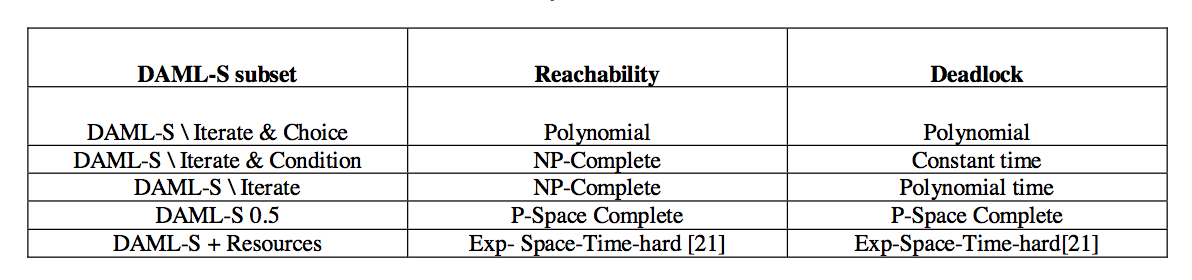
\includegraphics[width=1.2\columnwidth]{DAML-S-evaluation.png}
    \caption{Tractability results for DAML-S subsets}
    \label{fig:Conditional effects and outputs}
\end{figure}